\documentclass[10pt]{beamer}
\usepackage[french]{babel}
\usepackage[utf8]{inputenc}
\usepackage{graphicx}
\usepackage {mathtools}
\usepackage{utopia} %font utopia imported
\usetheme{CambridgeUS}
\usecolortheme{dolphin}


% set colors
\definecolor{myNewColorA}{RGB}{228,38,24}
\definecolor{myNewColorB}{RGB}{245,173,170}
\definecolor{myNewColorC}{RGB}{248,240,236}
\setbeamercolor*{palette primary}{bg=myNewColorC}
\setbeamercolor*{palette secondary}{bg=myNewColorB, fg = white}
\setbeamercolor*{palette tertiary}{bg=myNewColorA, fg = white}
\setbeamercolor*{titlelike}{fg=myNewColorA}
\setbeamercolor*{title}{bg=myNewColorA, fg = white}
\setbeamercolor*{item}{fg=myNewColorA}
\setbeamercolor*{caption name}{fg=myNewColorA}
\usefonttheme{professionalfonts}
\usepackage{natbib}
\usepackage{hyperref}
%------------------------------------------------------------
\titlegraphic{
\includegraphics[height=.5cm]{logo.png}}

\setbeamerfont{title}{size=\large}
\setbeamerfont{subtitle}{size=\small}
\setbeamerfont{author}{size=\small}
\setbeamerfont{date}{size=\small}
\setbeamerfont{institute}{size=\small}
\title[Spezialsuchmaschine]{Spezialsuchmaschine}
\subtitle{TP Web Sémantique}
\author[H4302]{H4302}

\institute[]{ INSA Lyon

Département Informatique}
\date[\today]
{\today}

%------------------------------------------------------------
\AtBeginSection[]{
  \begin{frame}
  \vfill
  \centering
  \begin{beamercolorbox}[sep=8pt,center,shadow=true,rounded=true]{title}
    \usebeamerfont{title}\insertsectionhead\par%
  \end{beamercolorbox}
  \vfill
  \end{frame}
}

\begin{document}

% Page de titre
\frame{\titlepage}

% Table des matières
\begin{frame}
\frametitle{Sommaire}
\tableofcontents
\end{frame}

%------------------------------------------------------------
\section{Introduction}
\begin{frame}{Introduction}
\begin{itemize}
    \item Présentation du projet : \textbf{Spezialsuchmaschine} est une application permettant de rechercher et d’afficher les marques automobiles allemandes ainsi que leurs modèles.  
    \item Objectif principal : Expérimenter l'utilisation du Web Sémantique via des requêtes \textit{SPARQL} sur DBpedia.
    \item Technologies utilisées :  
        \begin{itemize}
            \item HTML/CSS pour l'interface utilisateur.  
            \item JavaScript pour les requêtes dynamiques et la logique.  
            \item SPARQL pour interroger DBpedia.  
        \end{itemize}
\end{itemize}
\end{frame}

%------------------------------------------------------------
\section{Fonctionnalités}
\begin{frame}{Fonctionnalités}
\begin{itemize}
    \item Affichage des marques : Liste des marques automobiles allemandes triées par ordre alphabétique.  
    \item Recherche interactive :
        \begin{itemize}
            \item Possibilité de rechercher un modèle ou une marque automobile allemande.
            \item Filtrage en fonction des lettres saisies par l'utilisateur.  
            \item Affichage dynamique des résultats grâce à JavaScript.  
        \end{itemize}
    \item Interface claire : Cartes interactives pour les modèles préféré de chaque membre ainsi que pour la page des marques.
\end{itemize}
\end{frame}

\begin{frame}{Page d'accueil}
\centering
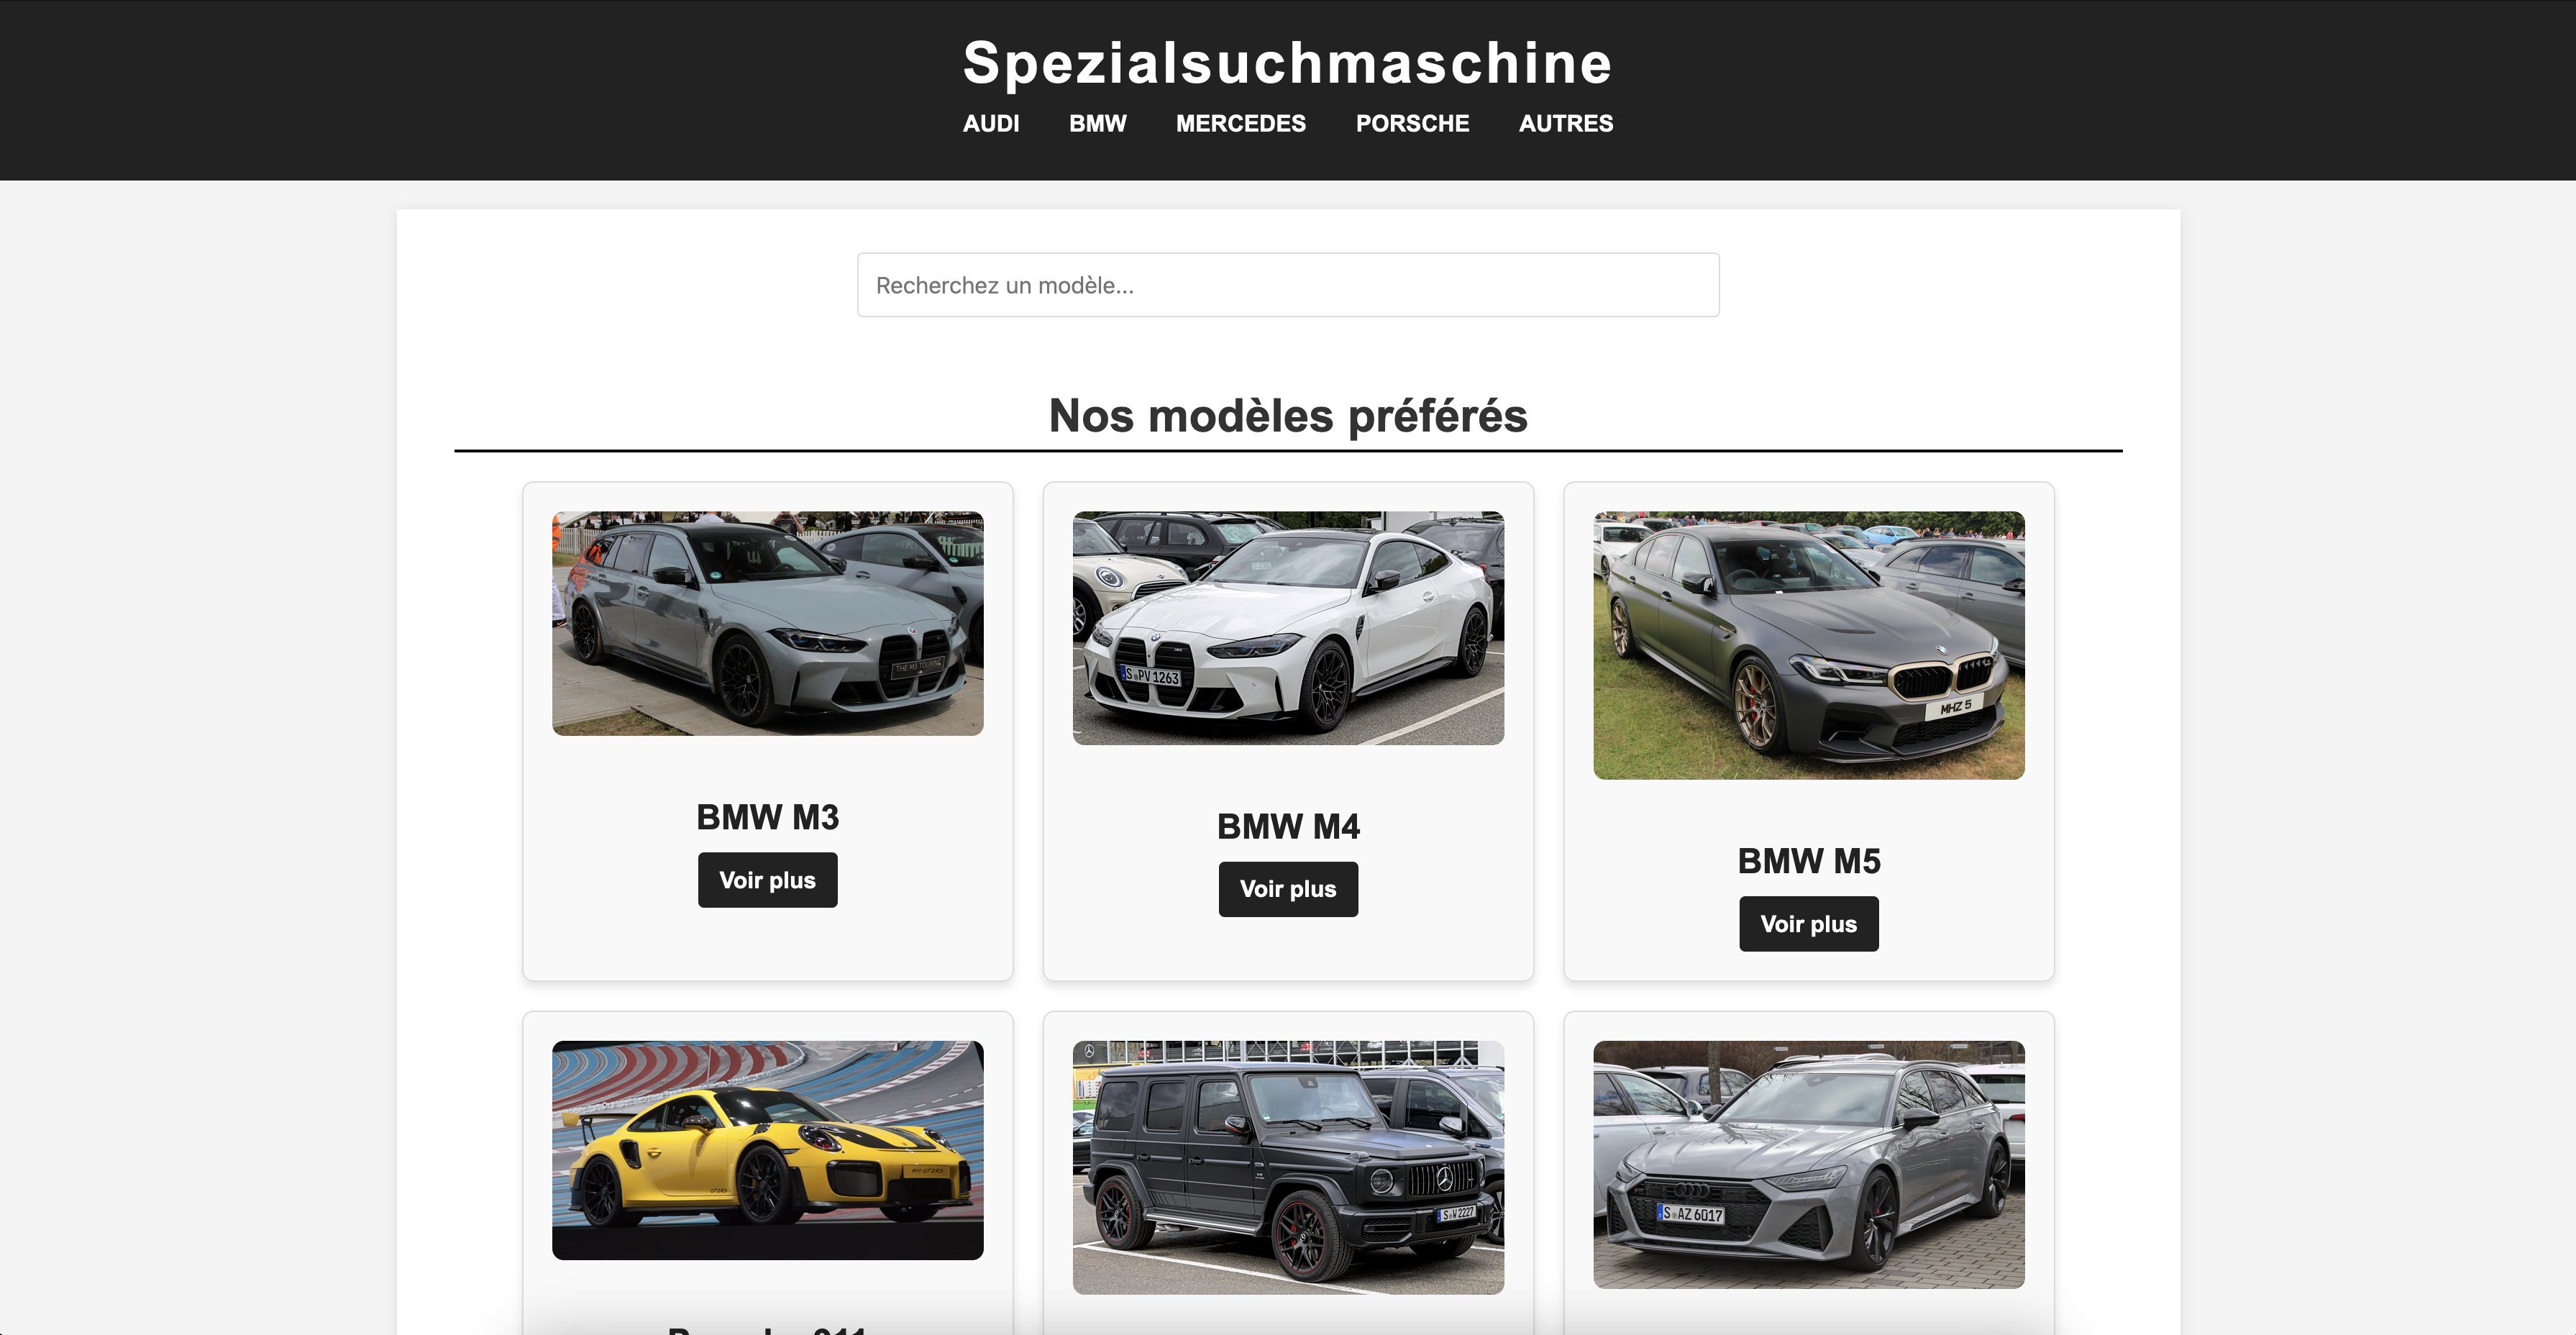
\includegraphics[width=0.8\textwidth]{images/index.png}
\end{frame}

\begin{frame}{Affichage des informations d'un modèle}
\centering
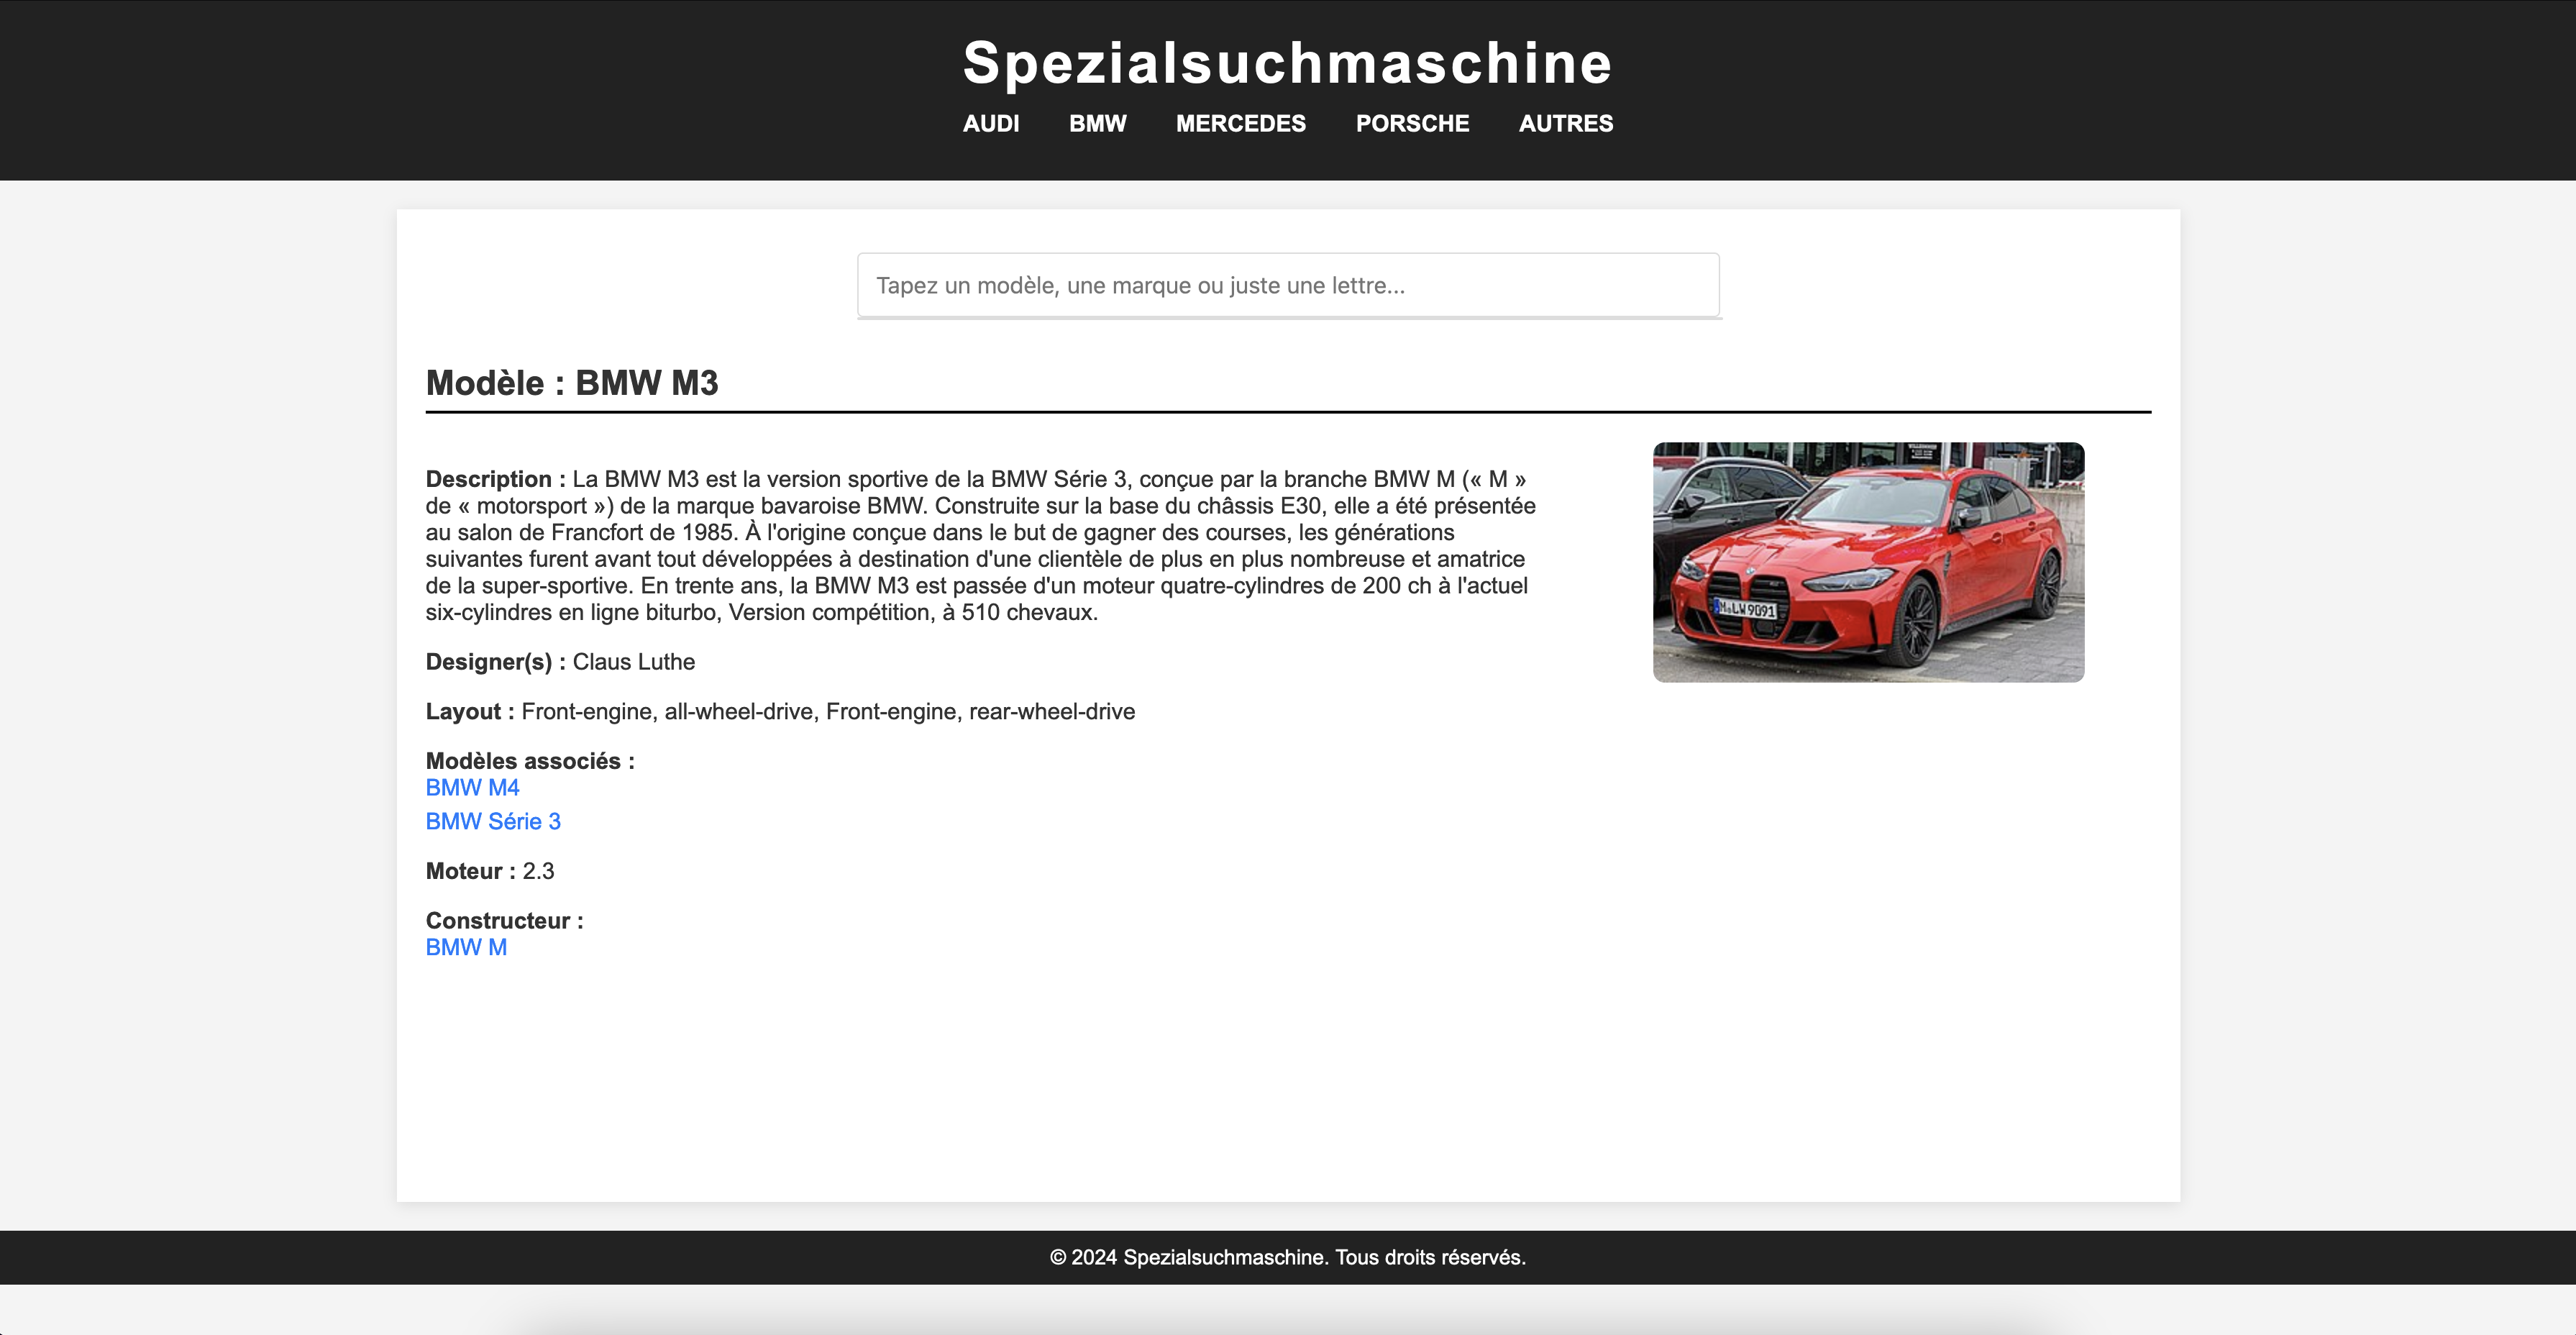
\includegraphics[width=0.8\textwidth]{images/modele.png}
\end{frame}

\begin{frame}{Affichage des informations d'une marque}
\centering
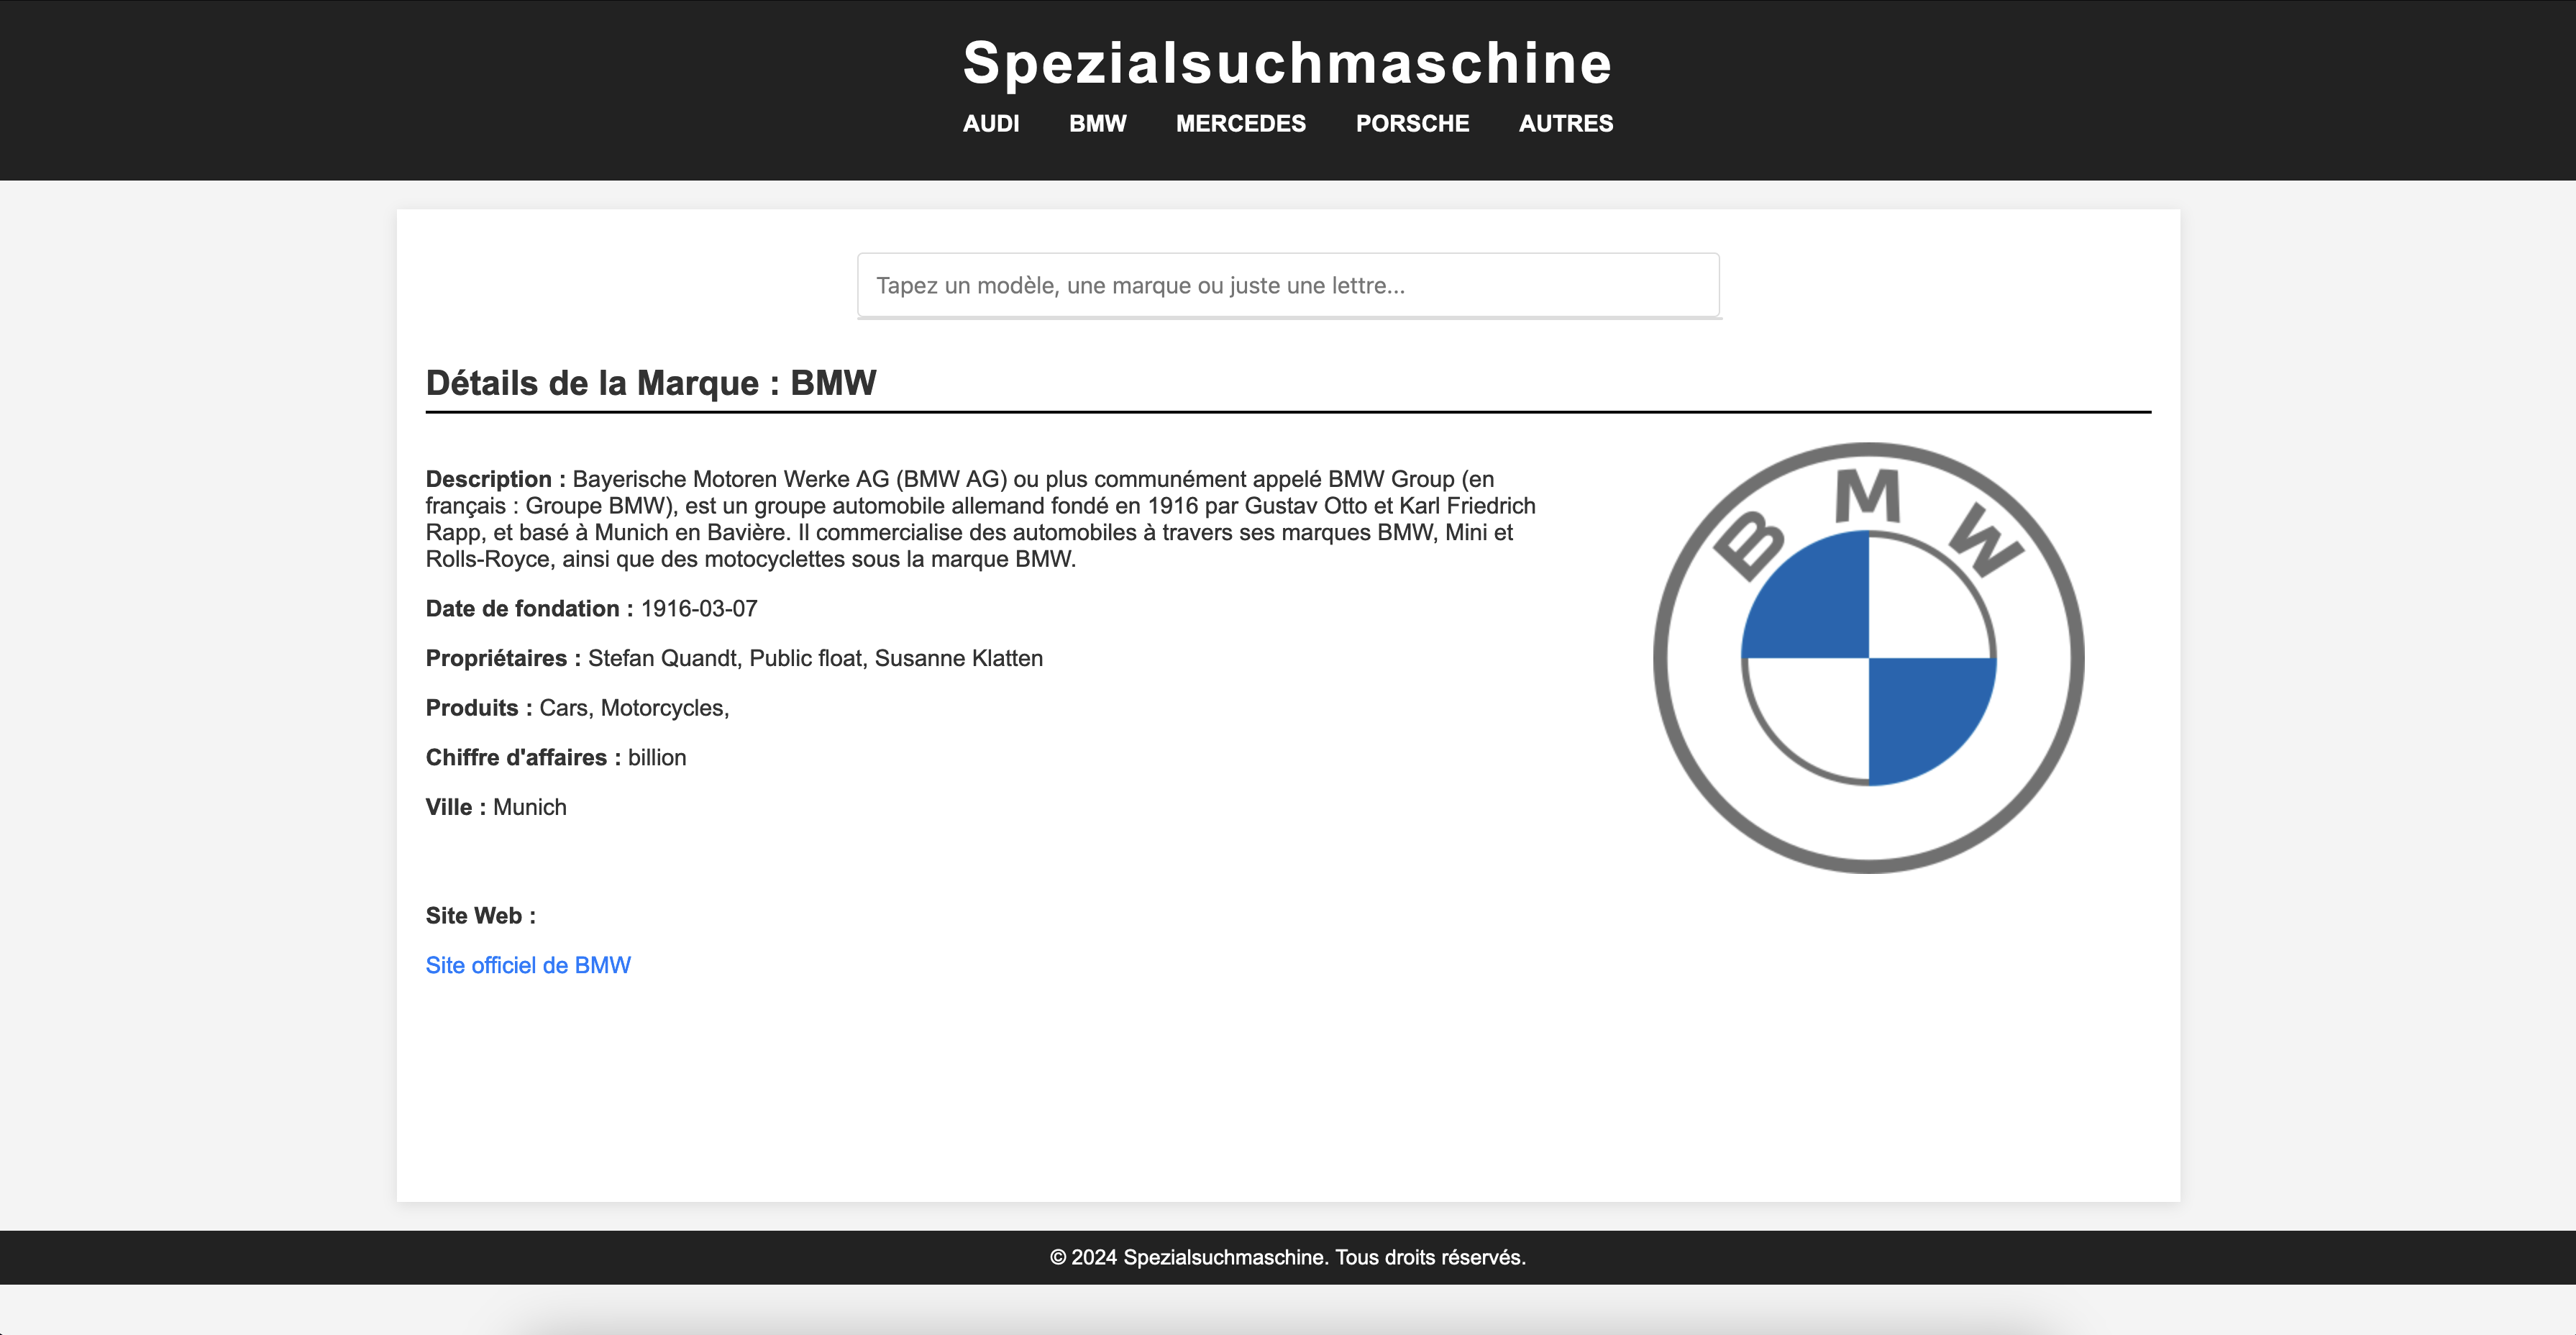
\includegraphics[width=0.8\textwidth]{images/marque.png}
\end{frame}

\begin{frame}{Affichage des marques automobile allemandes}
\centering
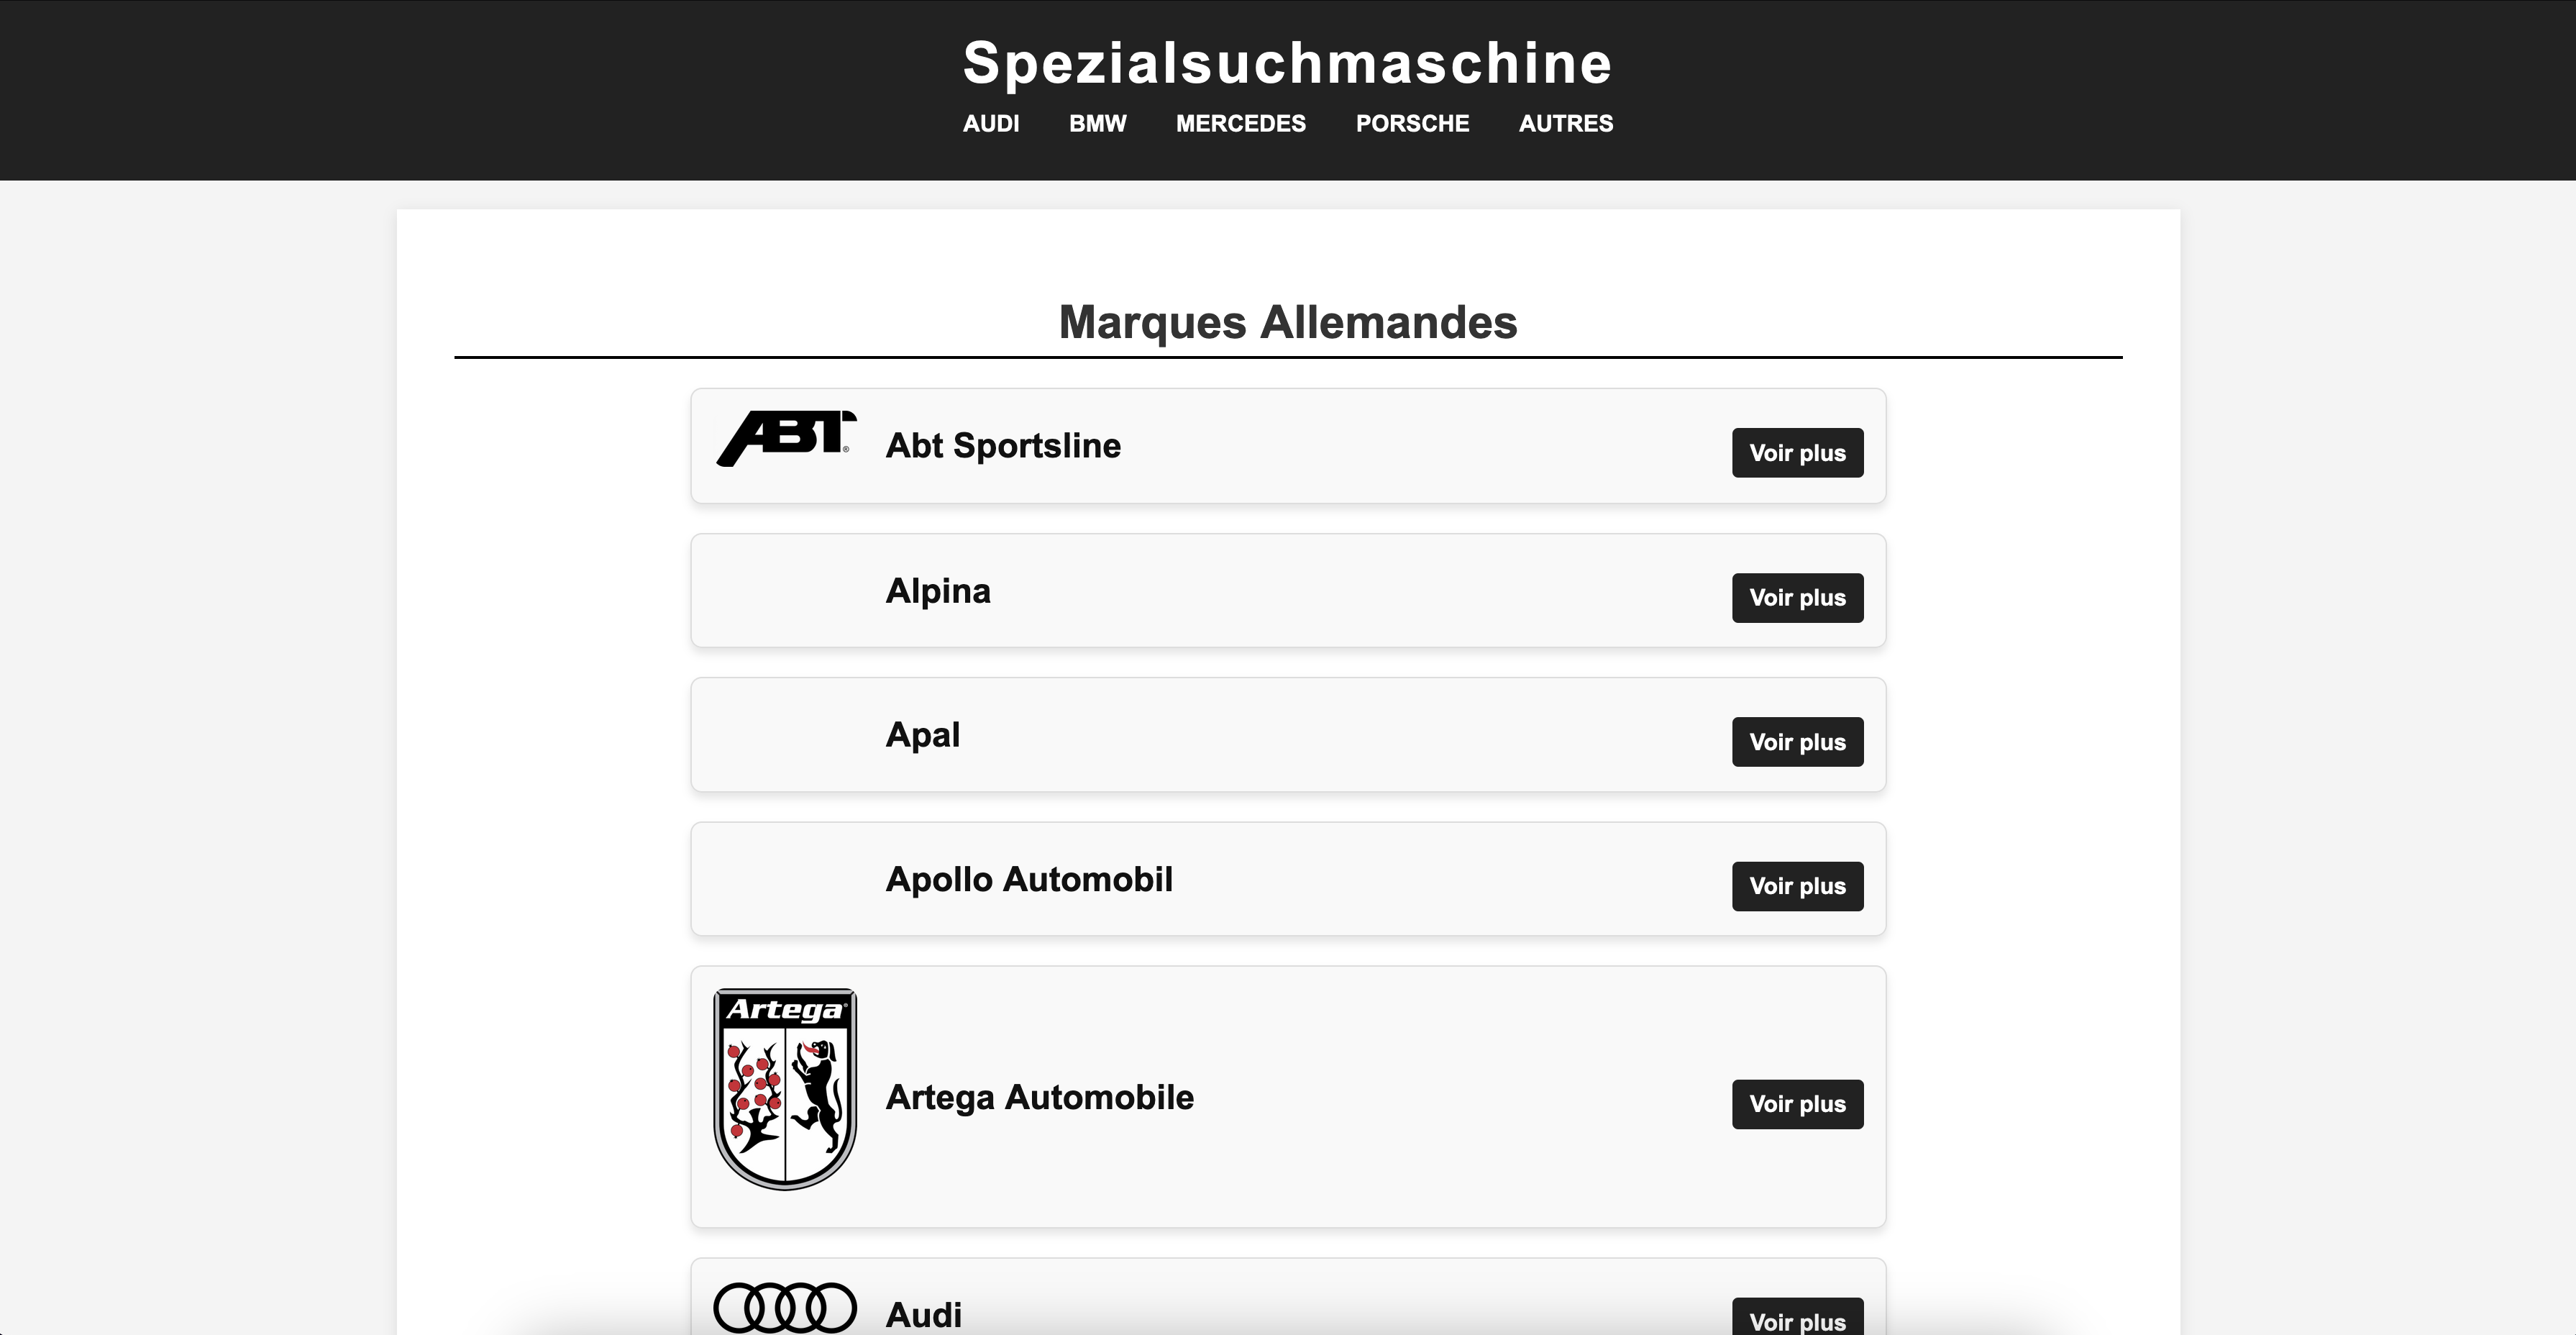
\includegraphics[width=0.8\textwidth]{images/marques.png}
\end{frame}

%------------------------------------------------------------
\section{Technologies utilisées}
\begin{frame}{Technologies utilisées}
\begin{itemize}
    \item \textbf{HTML/CSS} : Structure et mise en forme de l'interface.  
    \item \textbf{JavaScript} : Pour récupérer et afficher les résultats des requêtes SPARQL.  
    \item \textbf{SPARQL} : Requêtes pour extraire des données depuis DBpedia.  
    \item \textbf{DBpedia} : Source principale pour les données liées aux marques automobiles allemandes.  
\end{itemize}
\end{frame}

\begin{frame}[fragile]{Exemple de requête SPARQL}
Rechercher les modèles allemands commencant par "A" :
{\footnotesize
\begin{verbatim}
SELECT DISTINCT ?model ?modelLabel ?manufacturer ?manufacturerLabel
WHERE {
    ?manufacturer dct:subject dbc:Car_manufacturers_of_Germany .

    ?model (dbo:manufacturer|dbp:manufacturer) ?manufacturer .
    ?model rdf:type dbo:Automobile .

    ?model rdfs:label ?modelLabel .
    FILTER(LANG(?modelLabel) = "fr") .
    ?manufacturer rdfs:label ?manufacturerLabel .
    FILTER(LANG(?manufacturerLabel) = "fr") .
    FILTER(REGEX(STR(?modelLabel), "^A", "i")) .
}
LIMIT 5
\end{verbatim}
}
\end{frame}

\begin{frame}[fragile]{Exemple de requête SPARQL}
Rechercher les marques automobile allemandes commencant par "A" :  
{\footnotesize
\begin{verbatim}
SELECT DISTINCT ?manufacturer ?manufacturerLabel 
WHERE {
    ?manufacturer dct:subject dbc:Car_manufacturers_of_Germany .
    ?manufacturer rdfs:label ?manufacturerLabel .
    FILTER(LANG(?manufacturerLabel) = "en") .
    FILTER(REGEX(STR(?manufacturerLabel), "^${userInput}", "i")) .
}
ORDER BY ASC(?manufacturerLabel) 
LIMIT 5
\end{verbatim}
}
\end{frame}

\begin{frame}[fragile]{Exemple de requête SPARQL}
Obtenir la ville où BMW est implantée:
{\footnotesize
\begin{verbatim}
SELECT DISTINCT ?locationCity ?locationCityName
WHERE {
OPTIONAL {
    <http://dbpedia.org/resource/BMW> dbp:locationCity ?locationCity .
    ?locationCity rdfs:label ?locationCityName .
    FILTER(LANG(?locationCityName) = "en") .
    }
    OPTIONAL {
    <http://dbpedia.org/resource/BMW> dbo:location ?locationCity .
    ?locationCity rdfs:label ?locationCityName .
    FILTER(LANG(?locationCityName) = "en") .
    }
}
\end{verbatim}
}
\end{frame}
%------------------------------------------------------------
\section{Réflexion sur le Web Sémantique}
\begin{frame}{Réflexion sur le Web Sémantique}
\begin{itemize}
    \item Avantages :  
        \begin{itemize}
            \item Accès à des données structurées et interconnectées.  
            \item Utilisation de SPARQL pour des requêtes complexes.  
        \end{itemize}
    \item Inconvénients / Problèmes rencontrés :  
        \begin{itemize}
            \item Dépendance à une source externe (DBpedia).  
            \item Temps de réponse variable et risque d'indisponibilité.  
            \item Syntaxe SPARQL parfois complexe pour des débutants.  
        \end{itemize}
\end{itemize}
\end{frame}

%------------------------------------------------------------
\section{Conclusion}
\begin{frame}{Conclusion}
\begin{itemize}
    \item \textbf{Bilan} : Création réussie d'une application fonctionnelle exploitant le Web Sémantique.  
    \item \textbf{Compétences acquises} :  
        \begin{itemize}
            \item Utilisation de SPARQL pour interroger des bases de données sémantiques.  
            \item Intégration dynamique des résultats avec JavaScript.  
            \item Conception d'une interface ergonomique avec HTML/CSS.  
        \end{itemize}
    \item \textbf{Perspectives} :  
        \begin{itemize}
            \item Ajouter des détails supplémentaires pour chaque marque (images, historique).  
            \item Explorer d'autres sources de données liées au Web Sémantique.  
        \end{itemize}
\end{itemize}
\end{frame}

%------------------------------------------------------------
\section*{Acknowledgement}
\begin{frame}
\textcolor{myNewColorA}{\Huge{\centerline{Merci pour votre attention !}}}
\end{frame}

\end{document}